\chapter{HomeDS - Server}
\section{Einleitung}\label{sec:einleitung}
Im Rahmen der Diplomarbeit wird neben dem XIBO-Server ein weiterer Server eingesetzt. Es handelt sich um einen Java Enterprise Edition Server. Aufgrund der hohen komplexität des Signage-Servers aber jedoch dünn dokumentierten API-Schnittstellen und begrenzten technischen Möglichkeiten, muss ein eigens programmierter Server eingesetzt werden. Dieser wird die Kommunikation vom Signage Server zur Android App erleichtern. Der JavaEE Server verwendet die Funktionen des Signage Servers und baut diese meist aus sodass neue Funktionen entstehen können.

GRAFIK KOMMUNIKATION
 
\section{Anforderungen an den HomeDS Server}\label{sec:homeds}
Der JavaEE Server soll die verschiedenen komplizierten Abläufe des XIBO-Servers vereinfachen. Die  Zugriffe mittels REST die eigentlich direkt auf den XIBO laufen sollen, werden über den JavaEE Server verwaltet. Das heißt der Java Enterprise Server empfängt REST Zugriffe verarbeitet diese entsprechend und tätigt dann REST Abfragen auf den XIBO Server. Dies hat insofern Vorteile, da die komplizierten und meist mit viel Aufwand verknüpften Authentifizierungen wegfallen. Somit können ohne Probleme neue Funktionen hinzugefügt und neue Anforderungen flexibel erfüllt werden. Unser System erweitert  den Signage Server.
 
\section{Komponenten des HomeDS Server}\label{sec:homedscomponents}
Der JavaEE Server verfügt über eine eigene MySQL Datenbank. Diese wird benötigt, um Nachrichten Pakete und Kampagnen' aus dem Signage-Server zwischenzuspeichern. Diese Nachrichten Pakete auch DataSets genannt enthalten einen Titel und eine Nachricht die dann angezeigt werden. Des weiteren ist auf dem Server auch eine JSF also Java Server Faces Komponente dabei. Diese gibt den Nutzern die Möglichkeit über die HomeDs Webseite alle Funktionen des Server zu nutzen. Der ganze Server wird auf einem Wildfy Application Server mittels Continous Integration deployed. 
 
\section{Funktionen des JavaEE}
\subsection{DataSet mit Ablaufdatum}\label{sec:datasetexpiredate}
Eine der Funktionen des Servers ist das Hinzufügen, Ändern und Löschen von DataSets. Da der Digital Signage Server über keine Zeitsteuerung der Nachrichten Pakete verfügt musste diese Funktion auf den JavaEE Server ausgelagert werden.

Der Benutzer kann Start- und Enddatum für jeden einzelnen DataSet eingeben. Erst wenn das Datum genau in diesem Zeitintervall inklusive den Grenzen liegt, wird das DataSet an den Xibo mittels API-Schnittstelle weitergegeben. Es wurde auch so programmiert das bei keinem Startdatum das Nachrichten Paket sofort angezeigt wird oder wenn kein Enddatum festgelegt wird das es bis zum Manuellen deaktivieren angezeigt wird.

\begin{lstlisting}[language=Java, caption={public void doCheckEvery24Hours()}]
if (dataset.isActive() == false && (dataset.getFromDate().minusDays(1)
        .isBefore(LocalDate.now()))) {
    try {
        //if succesfull added then set active true and add id
        if ((id=dataSetApi.addDataSetField(dataset)) > 0) {
            dataset.setDataRowId(id);
            dataset.setActive(true);
            dataSetFieldFacade.save(dataset);
        }
    } catch (NoConnectionException e) {
        // Catch Exception
    }
}
\end{lstlisting}

Die Überprüfung ob die DataSets aus der Server-Datenbank im Zeitintervall liegen, wird mithilfe der Java Annotation @Schedule jeden Tag um 01:00 Uhr durchgeführt. Falls dieses DataSet im Intervall liegt, wird dieses an den XIBO Signage Server gesendet. Diese Überprüfung beinhaltet auch das FromDate. Dies löscht bei überschreiten des Bis-Datums das DataSet aus dem Digital Signage heraus. Solange das DataSet sich im XIBO befindet wird es angezeigt nach dem entfernen aus dem XIBO wird es dann auch nicht mehr angezeigt.

Falls keine Nachrichten Pakete aktiv oder im System sind werden aus dem RSS-Feed der HTL Leonding die Neuigkeiten anstatt der Nachrichten Pakete angezeigt.

\subsection{Medien abspielen}\label{sec:playmedia}
Eine weitere Funktion des Servers ist das abspielen von Medien auf einen bestimmten Bildschirm. Dabei muss im XIBO ein definiertes Layout erstellt werden mit einer absoluten Id. In diesem Layout wird eine Region über die volle Auflösung erstellt die ein Bibliothek Widget enthält. Diesem Widget wird dann per REST das vom Nutzer ausgewählt Medium eingefügt. Sobald diese Operationen erfolgreich ausgeführt wurden wird per REST das definierte Layout auf den vom Nutzer ausgewähltem Bildschirm eingeplant.

\subsection{Jave Enterprise Edition mit Android über REST}\label{sec:javaeeandroidrest}
Ein weiterer Teil des Server auf Java Enterprise Edition Basis ist die Kommunikation mittels REST. Alle Funktionen des Servers werden per REST zur Verfügung gestellt.

\subsection{Swagger}\label{sec:javaeeandroidrestswagger}
Swagger wird verwendet um Funktionalität und Möglichkeit einer API übersichtlich zu gestalten. Dabei gibt es zwei verschiedene Arten eine REST-Dokumentation zu erstellen.
Dabei dokumentiert Swagger welche Response Code's man erwarten kann wie bei einem POST oder PUT der Body aussehen muss oder welche Pathparams mitgegeben werden müssen und welche nur optional sind.  

Die erste Möglichkeit wäre, mit dem Swagger Editor die Dokumentation in der JSON-Ausdruckssprache mit der Hand zu schreiben und immer wieder zu aktualisieren. Natürlich ist dies bei vielen verschiedenen GETs, POSTs, PUTs und DELETEs sehr aufwendig und mühsam.

Bei der zweiten Methode, die auch bei der Diplomarbeit zum Einsatz kommt, werden die API's automatisch von der im Projekt eingebundenen Swagger Engine erkannt. Daraus wird dann auch wieder eine JSON-File generiert, die dann mithilfe von Swagger-UI gut im Browser über eine Webseiten URL erreichbar ist.


Verweis: https://swagger.io/

\section{Java Server Faces mit JavaEE}\label{sec:javaeejsf}
Um den Benutzern die Möglichkeit zu geben die Funktionen unseres Servers zu nutzen wurde im Rahmen der Diplomarbeit auch eine Webapplikation erstellt. Und da JSF also Java Server Faces mit einem Java EE Server harmoniert haben wir uns entschieden solch eine Webapplikation zu erstellen. Dies hat viele Vorteile wie z. Bsp. die Platformunabhängigkeit und auch die schnelle Entwicklung im Vergleich zu anderen Clients. 

Mit JSF wird nämlich über eine Managed Bean direkt im XHTML auf die Funktionen des Servers zugegriffen somit sind keine REST Zugriffe nötig.

\begin{figure}[h]
\centering
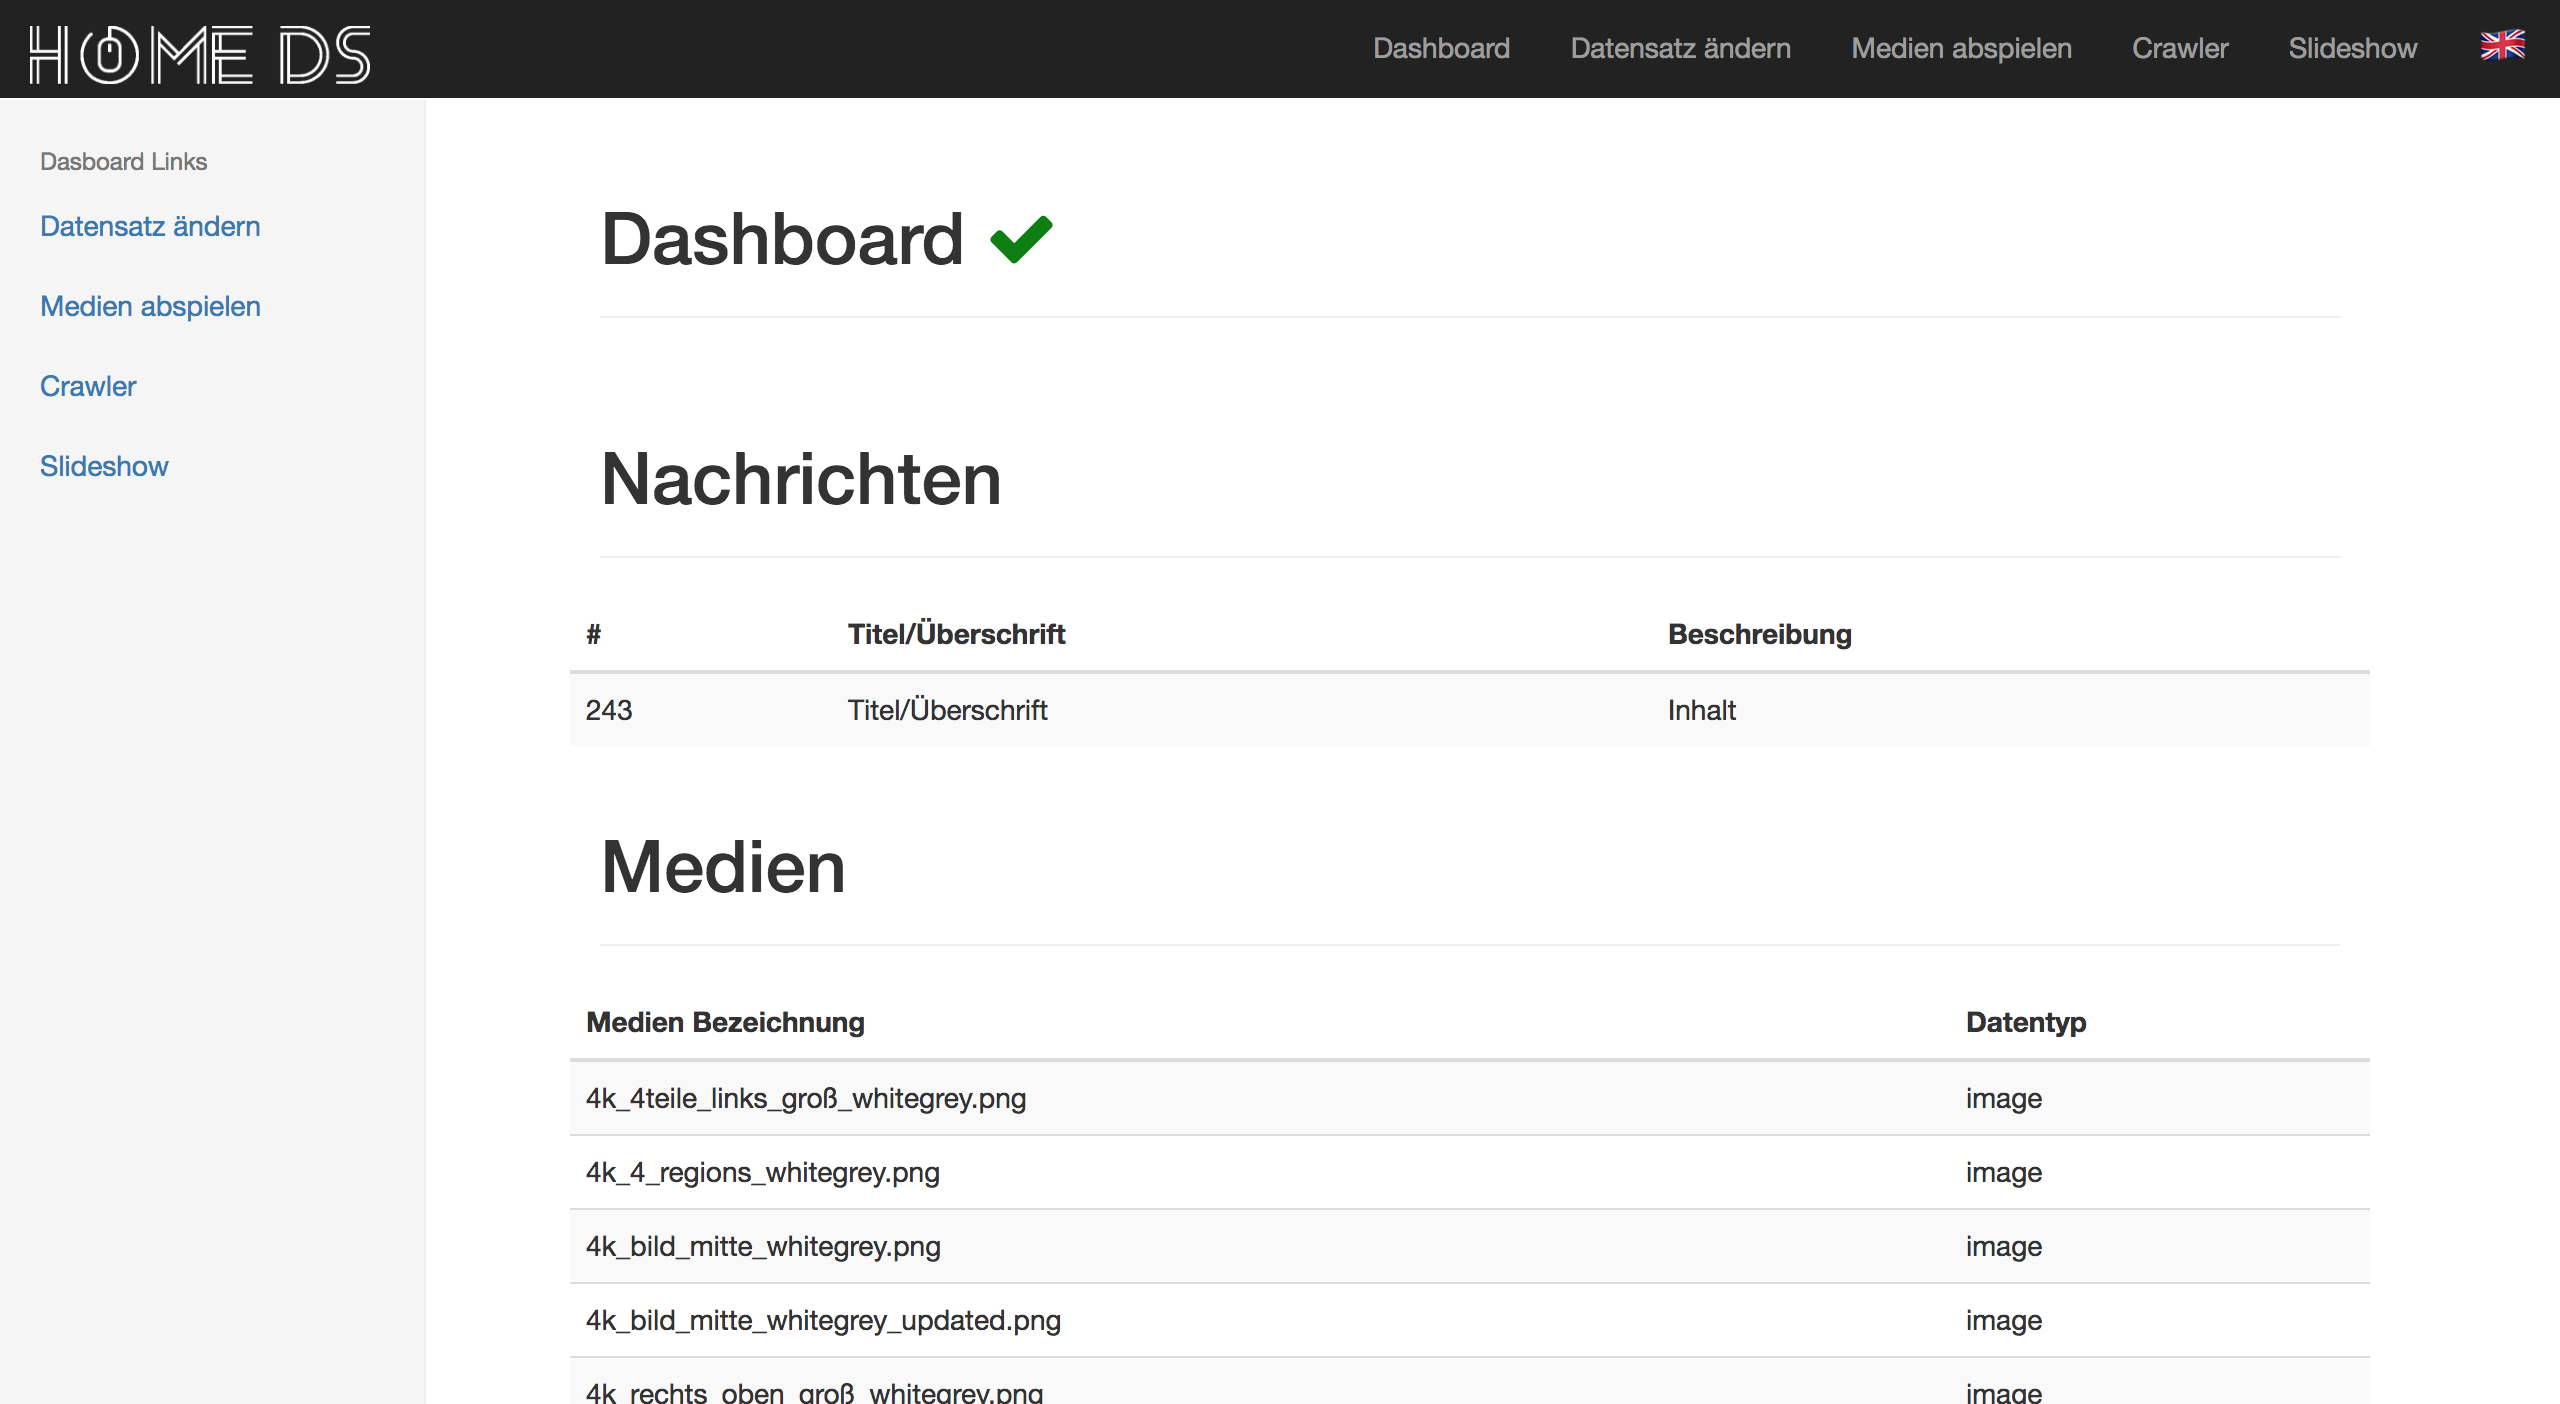
\includegraphics[width=1\textwidth]{images/08_HomeDsWeb/DashboardHomeDsWeb.png}
\caption{Startseite - HomeDsWeb}
\label{img:Startseite}
\end{figure}

Unsere Weboberfläche ist Responsive gestaltet und mithilfe von Java Server Faces mit BootsFaces realisiert worden. Das Bootsfaces Framework stellt fertige Komponenten zur Verfügung wie Buttons, Listen, Forms etc. Dabei wurde Bootstrap als Vorbild hergenommen.

Uns war es wichtig die Oberfläche so zu gestalten das diese übersichtlich und leicht zu bedienen ist. Das Designen wurde mit enger Zusammenarbeit mit dem zukünftigen Benutzern der Software ausgearbeitet. Als Vorbild fungierte mehr oder weniger ein Cockpit eines Flugzeuges wo vielen Funktionen direkt bei der Hand liegen müssen und trotzdem alles seine Ordnung hat. In der Abbildung \ref{img:Startseite} ist das Dashboard abgebildet. 
Hier erkennt man nun das es sich um die Kommandozentrale der Applikation handelt von dieser Seite aus kann man über eine Top-Navigationsleiste oder Left Sidebar Navigation zu allen Funktionen des Server gelangen. 

Um den Nutzer immer ein Feedback über den aktuellen Status der Verbindung vom XIBO zu JavaEE Server zu geben wird bei Erfolgreicher Verbindung ein grünes Häkchen visualisiert versehen mit eine Tooltip. Oder bei keiner Verbindung zum Server ein rotes x dargestellt wie in Abbildung  \ref{img:NoConnection}.

\begin{figure}[h]
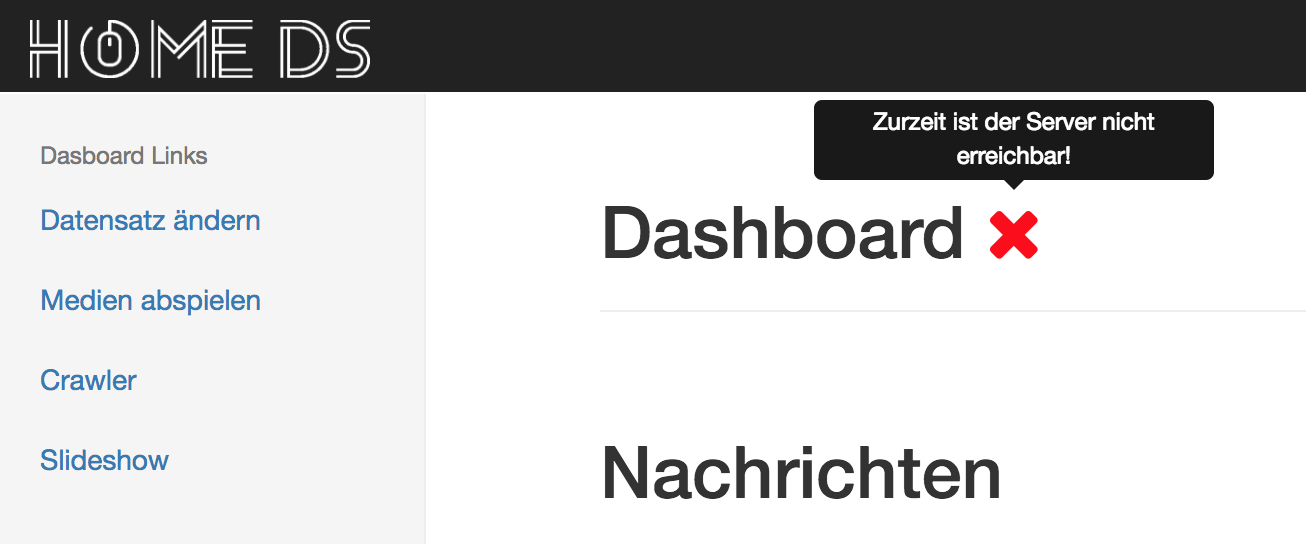
\includegraphics[width=1\textwidth]{images/08_HomeDsWeb/DashboardNoConnection.png}
\caption{Keine Verbindung zum XIBO - HomeDsWeb}
\label{img:NoConnection}
\end{figure}

\section{Nachrichten Pakete ändern - HomeDS Web}\label{sec:homedswebdataset}
Die Datensatz ändern Funktion auch genannt Nachrichten Pakete ändern, DataSet bearbeiten oder Nachrichten Pakete bearbeiten kann über das Dashboard erreicht werden.
Die Aufgabe der DataSet Webapplikation ist ein DataSet zu ändern, hinzufügen oder zu löschen. Die Applikation besteht grob gesagt aus 2 Teilen. Diese 2 Teile können bei Bedarf auf- und zugeklappt werden.

Teil 1 kümmert sich um das Anzeigen aller DataSets in einer Responisve Komponente die "DataTable" gennant wird in der Bibliothek vom Bootsfaces Framework. Im DataTable ist es möglich die Anzahl der angezeigten Elemente pro Seite zu begrenzen oder erweitern,  die einzelnen Spalten sortieren dabei kann man zwischen ab- oder aufsteigend wählen und durch die verschiedenen Spalten einer Zeile eine Suche durchzuführen. 

Es ist auch durch die editierbaren Textfelder und DatePicker möglich die DataSets zu ändern. Durch klicken auf den Speichern Button wird die Änderung des einzelnen DataSets bestätigt. Durch klicken auf den roten Löschen Button wird das Nachrichtenpaket gelöscht falls es aktiv war wird es auch aus dem XIBO System entfernt. Die Logik ist im \pageref{sec:datasetexpiredate} nochmals genauer erklärt. 

Der zweite Teil der Datensatz ändern Seite ist das Hinzufügen von Nachrichtenpaketen. Dabei ist der Titel und der Inhalt der Nachricht natürlich erforderlich. Bei nicht eingeben von Start Datum des Nachrichtenpakets wird davon ausgegangen das es sofort in den XIBO gespeichert werden soll und somit auf aktiv gesetzt wird. Andersrum wenn kein Ablaufdatum eingegeben wird, wird das DataSet solange angezeigt bis entweder ein Ablaufdatum im Nachhinein hinzugefügt wird oder es manuell einfach wieder gelöscht wird.

Nach jeder Aktion wird die Webseite mit einer Loading Animation versehen und der Nutzer bekommt dann ein Feedback ob die jeweilige Operation erfolgreich oder fehlgeschlagen ist. 

Verweis auf JSF Section,


\section{Medien abspielen}\label{sec:playmedia}
Eine weitere Funktion ist das Abspielen der Medien die im XIBO hinterlegt sind. Es soll dem Nutzer eine einfache und übersichtliche Oberfläche zur Verfügung gestellt werden die Medien abspielen soll. Der Nutzer kann jedoch vorher den Bildschirm auswählen auf den diese Medien abgespielt werden sollen. Des weiteren soll verhindert werden das der Nutzer stundenlang sein gewolltes Video aus der XIBO Bibliothek heraussuchen muss. Diese Herausforderung wurde mithilfe von Schlagworten und einer Schlagwort-Wolke gelöst. Auch werden nur Formate wie Foto und Video aus der XIBO Bibliothek geladen.

\begin{figure}[h]
\centering
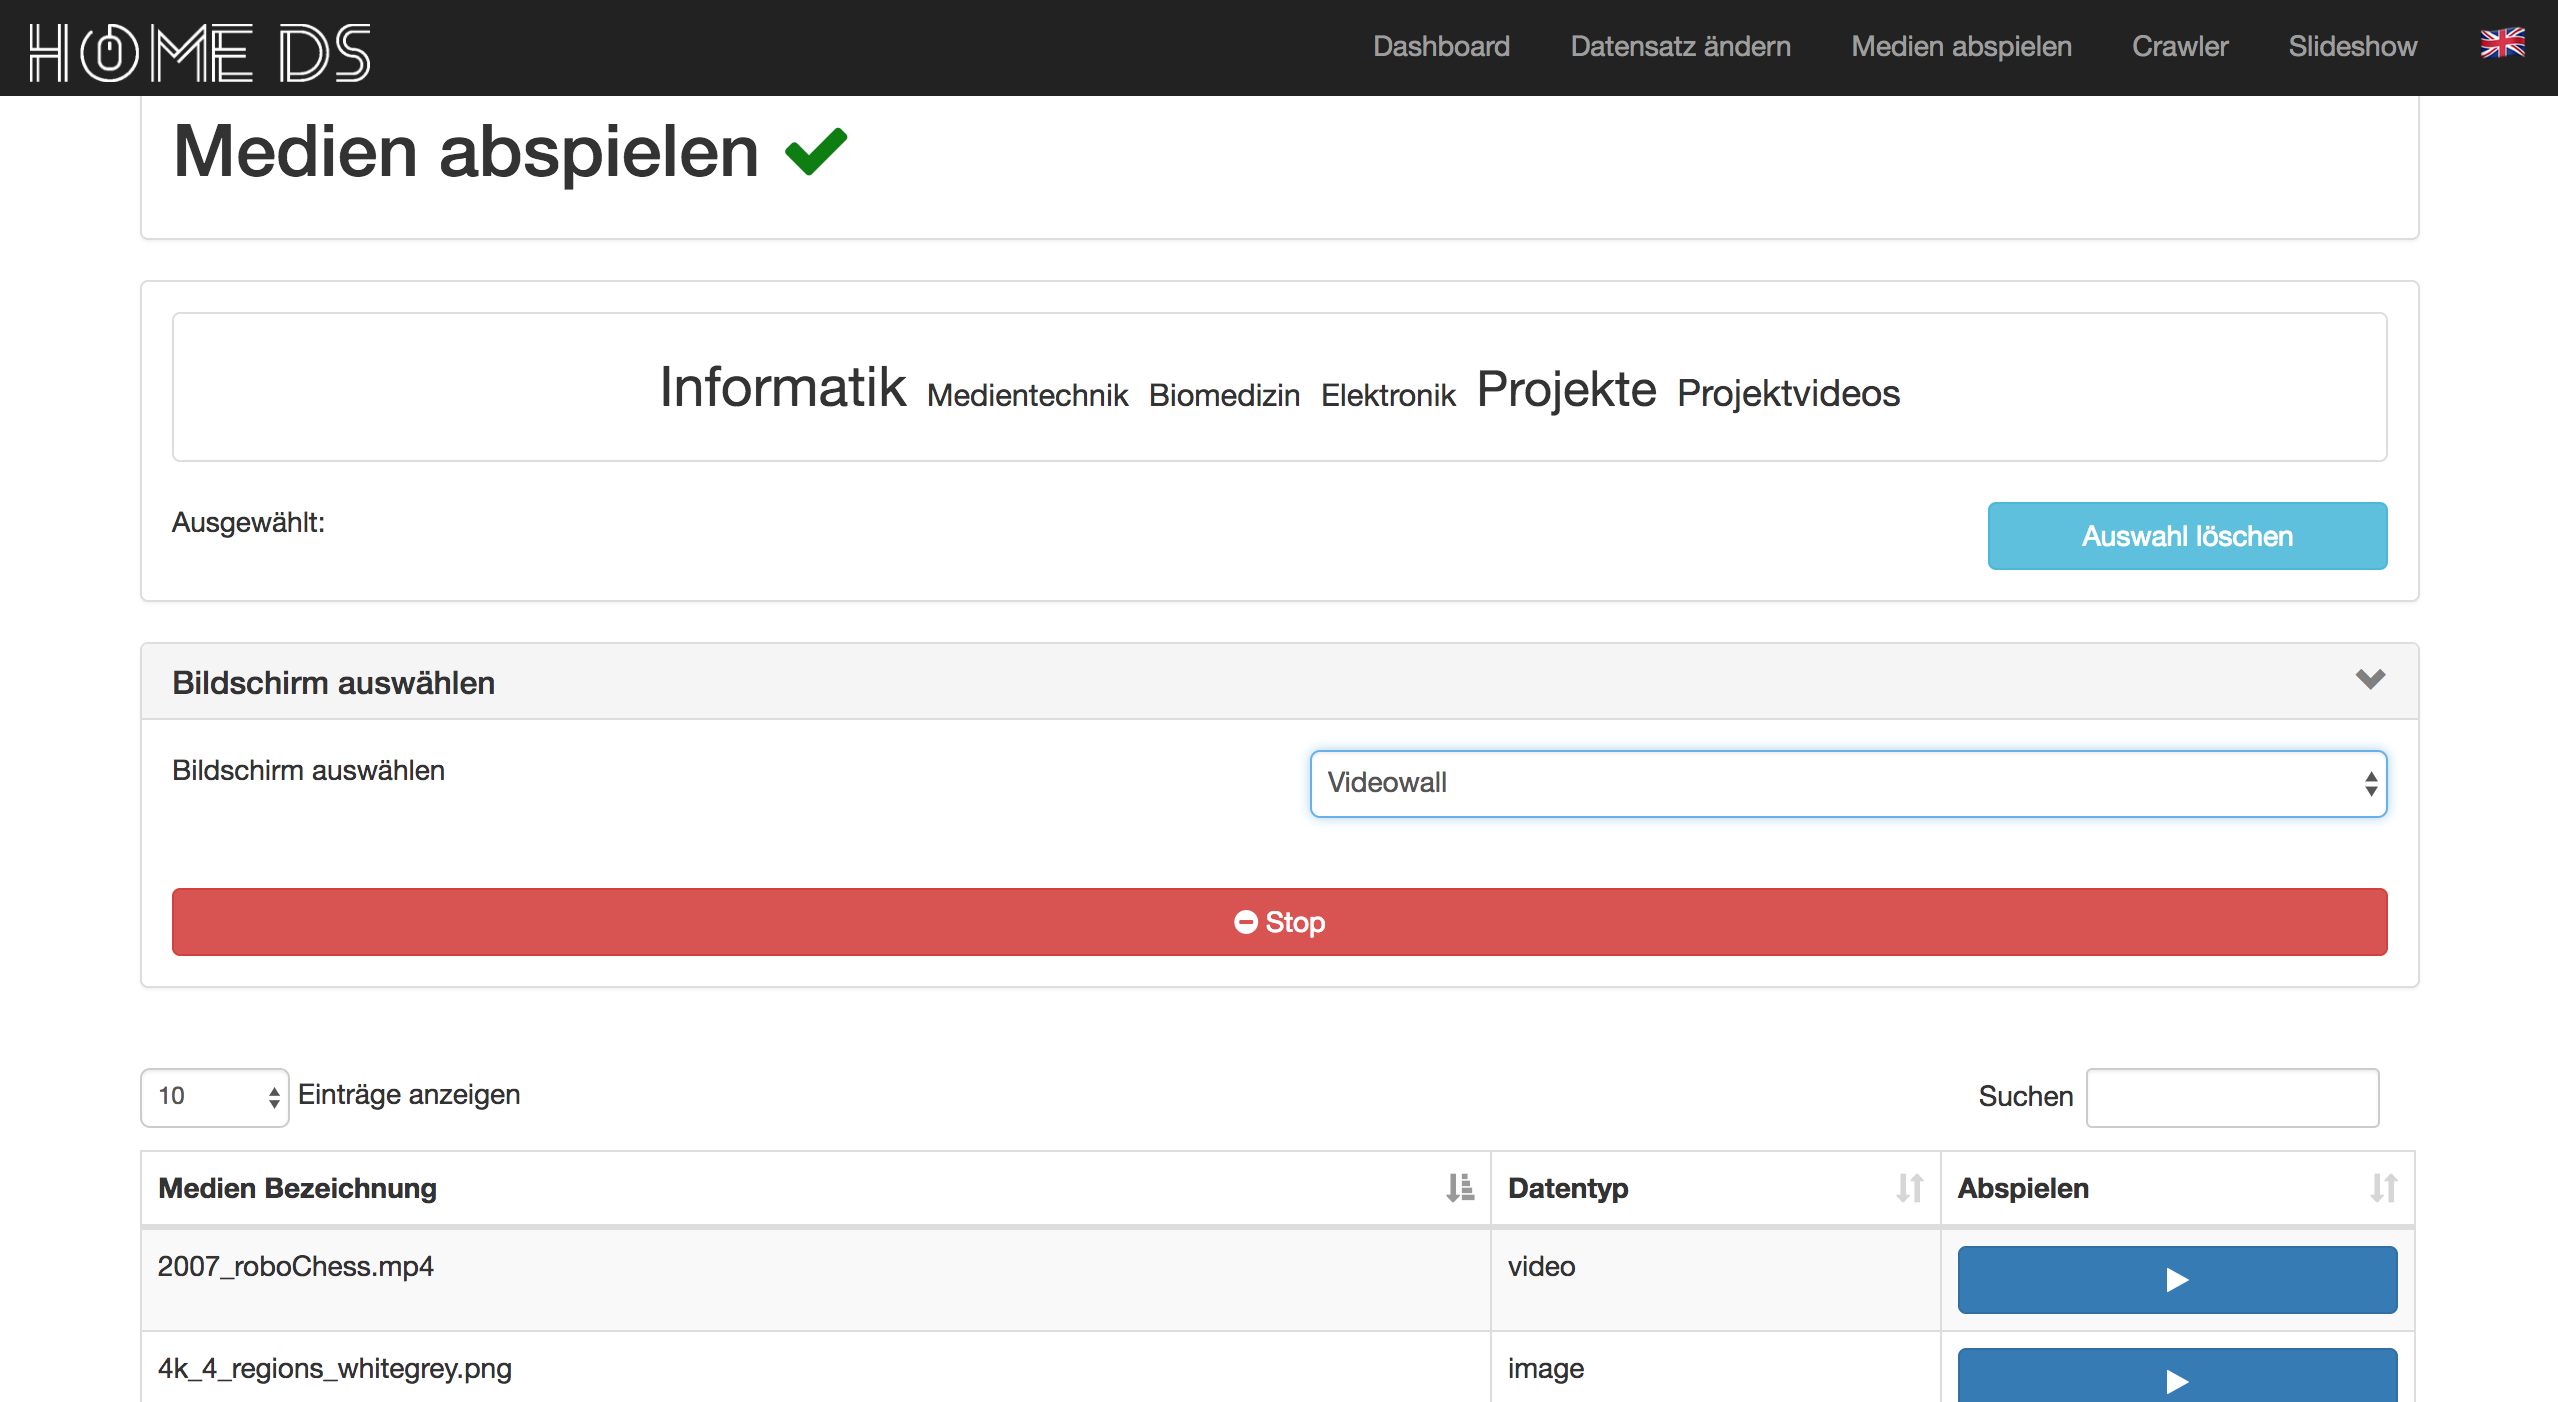
\includegraphics[width=1\textwidth]{images/08_HomeDsWeb/PlayMediaOverview.png}
\caption{Medien abspielen- HomeDsWeb}
\label{img:playmedia}
\end{figure}

Die Medien im XIBO müssen mit einem Schlagwort versehen. Diese Schlagwörter können sein die jeweilige Abteilung also Informatik, Medientechnik oder Elektronik. Oder aber auch ob es sich um ein Projekt oder sonstiges. Siehe Abbildung \ref{img:playmedia}

Mithilfe dieser Tags wollen wir dem Nutzer die Suche nach dem richtigen Video erleichtern. Der Nutzer bekommt die Möglichkeit einer dieser Tags auf der HomeDs Weboberfläche auszuwählen daraufhin werden nur die Videos mit dem entsprechendem Tag angezeigt.

So nachdem der Nutzer sein Schlagwort und den gewünschten Bildschirm ausgewählt hat und auch schon das Video oder Foto gefunden hat welches er anzeigen möchte muss er nur den Play-Button drücken. Nach der Meldung das dieses Element erfolgreich abgespielt wurde erscheint es innerhalb weniger Sekunden auf dem gewünschten Bildschirm. Das Video wird bis zum Ende abgespielt und dann wieder das vorige Layout hergestellt. Wenn ein weiteres Element abgespielt während dem Element 1 wird das Video 1 abgebrochen und das Element 2 wird abgespielt.

Neben dem Abspielen gibt es auch die Stop Funktion diese soll sofort wieder das Layout vor dem Abspielen des Videos anzeigen.


\section{HomeDS Server Projekt-Struktur}\label{sec:javaeestruktur}


\section{HomeDS Server Structure Crawler}\label{sec:javaeestructurecrawler}
Für das verstehen des Aufbaus eines Layouts war es die Aufgabe einen sogennanten StructureCrawler zu erstellen. Dieser soll den JSON Aufbau eines Layouts ausgeben. Durch diese Funktion ist es für uns möglich gewesen das ganze Signage System zu verstehen und zu verwenden. Der Crawler ist eigentlich nur ein REST-Zugriff der sich alle Layouts vom XIBO Server holt und dabei alle anderen Child-Elemente des Layouts mitschickt. Dies ist praktisch den es unterstützt uns bei dem Arbeiten mit vielen verschiedenen Ids die richtig sein müssen.

WEBOBERFLÄCHE VOM CRAWLER

\section{HomeDS Server Slideshow}\label{sec:homedsslideshow}
Eine weitere Funktion des HomeDs Servers ist das abspielen von Medien ohne diese in den XIBO hochladen zu müssen. Dies ist insofern wichtig da man bei großen Mengen von Daten nicht das XIBO zu müllen sollte. Dies wurde mittels JSF, Bootsfaces und JavaScript realisiert. Die Bilder werden von einem lokalen Ordner der Reihe nach abgespielt. Der Wechselintervall beträgt 3 Sekunden.

JavaScript	code erklären
